\subsection{字符串匹配}
%----------------------------------------------------------------------------------------
%	 CONTENT
%----------------------------------------------------------------------------------------
概念:
\begin{itemize}
\item 有效位移: 若子字符串(亦称为模式) $P$ 在文本 $T$ 中出现切位移为 $s$, 则称 $s$ 为有效位移, 否则为无效位移
\item 字符串匹配: 在一段指定的文本 $T$ 中找出某指定模式 $P$ 出现的所有有效位移
\end{itemize}

\begin{table}[h]
    \centering
    \begin{tabular}{lcc}
        \hline
        算法 & 预处理时间 & 匹配时间 \\
        \hline
        朴素算法 & 0 & O{((n - m + 1) m)} \\
        Rabin-Karp & $\Theta$(m) & O((n - m + 1) m) \\
        有限自动机 & O(m$|\sum|$) & $\Theta$(n) \\
        KMP & $\Theta$(m) & $\Theta$(n) \\
        \hline
    \end{tabular}
\caption{时间对比, 其中 $n,m$ 分别表示 $T,P$ 的长度; $\Theta,O$ 分别表示最坏情况下、平均情况下的时间估计; $\sum$ 表示 $T$ 的字符集合}
\end{table}

\section*{朴素算法}

思路: 用一个包含模式的``模板"沿文本滑动, 同时对每个位移注意模板上的字符是否与文本中的相应字符相等. 

\begin{figure}[h]
    \centering
    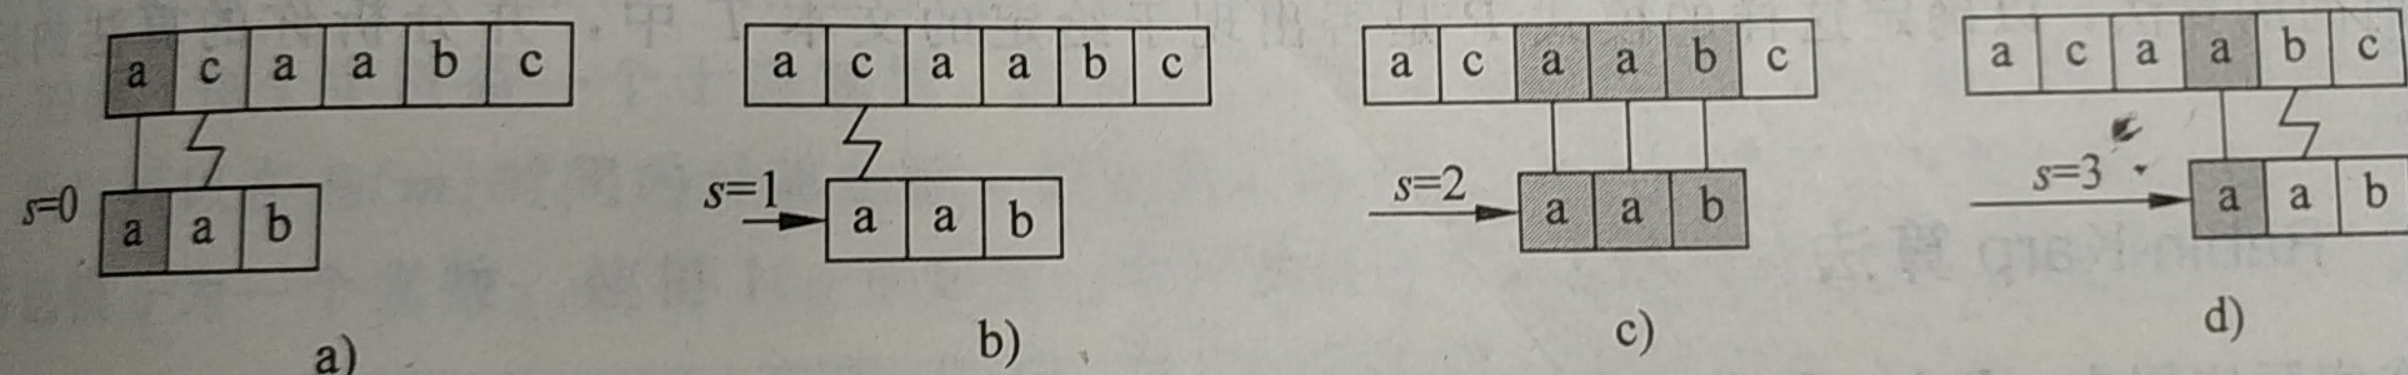
\includegraphics[height=2cm,width=14cm]{notes/algorithm/pic/朴素字符串匹配.png}
\end{figure}

\section*{Rabin-Karp}

思路: 将 $P,T$ 均转变成 $d$ 进制的整数 $p,t_s$, 其中 $s=0,1,\dots,n-m$, 然后直接比较 $p,t_s$ 是否相等即可找出所有有效位置 $s$. 具体做法下:
\begin{enumerate}
\item 预处理\
    \begin{itemize}
        \item 将$P$根据公式(\ref{eq:P})转变为$d$进制整数$p$(共需$\Theta(m)$时间) \
            \begin{equation}
                \begin{split}
                    p &= p_m \\
                    p_{i+1} &= P[i] + dp_i, \text{其中}p_0=0,i=0,1,\cdots,m-1 \label{eq:P}
                \end{split}
            \end{equation}
            此处 $P[i]$ 表示字符串 $P$ 从左边开始的第 $i$ 位字符. 由该公式可知, 在 $\Theta(m)$ 时间内即可完成 $P \to p$ 的转换. 同理, 在 $\Theta(m)$ 时间内将 $T[0 \dots m-1]$ 转换成 $t_0$
        \item 根据公式(\ref{eq:T}) $t_s$ 计算 $t_{s+1}$(共需$\Theta(n-m+1)$时间) \
            \begin{equation}
                t_{s+1} = d (t_s - d^{m-1} T[s+1]) + T[s+m+1] \label{eq:T}
            \end{equation}
            由该公式可知, $t_s \to t_{s+1}$ 可在常数时间$\Theta(1)$内完成
    \end{itemize}
\item 匹配: 若 $p$ 与 $t_s(s=0,1,\cdots,n-m)$ 相等, 则 $s$ 即为一个有效位置(每匹配一个候选有效位移,需要$\Theta(m)$时间,最坏情况下,每个位置均为候选有效位移,因此最坏匹配时间为$\Theta((n-m+1)m)$)
\end{enumerate}

公式($\ref{eq:T}$)处理时间为$\Theta(1)$的前提是: $p,t_s$的值不是很大. 若它们很大, 则公式($\ref{eq:T}$)则在常数时间内完成这一假设就不合理了. 解决该问题的方法是: 选取一个合适的模$q$来计算$p,t_s$的模, 若二者对应的模相等则说明$s$是一个候选有效位移, 然后直接比较字符串$P,T[s \dots s+m-1]$来判断$s$是否为有效位移. 因此, 改进后的公式(\ref{eq:P},\ref{eq:T})对应如下(\ref{eq:P2},\ref{eq:T2}):
\begin{equation}
    \begin{split}
        p &= p_{m-1} \\
        p_{i+1}  &= (P[i] + dp_i) \mod q, \text{其中}i=0,\cdots,m-1 \label{eq:P2}
    \end{split}
\end{equation}
\begin{equation}
    \begin{split}
        t_{s+1} &= \left(d(t_s - h T[s+1]) + T[s+m+1]\right) \mod q \\
        h &= d^{m-1} \mod q\label{eq:T2}
    \end{split}
\end{equation}
一般而言, 所选取的$q$为素数且满足$dq$在一个字节内, 即$2^8=256$内. 若 $q$ 足够大, 就可期望候选有效位移/伪命中点减少

\begin{algorithm}[htbp]
    \caption{Rabin-Karp(T,P,d,p)}
    \label{alg:rabin-karp}
    \begin{algorithmic}[1] % 显示行号
        \STATE $n \leftarrow length[T]; m \leftarrow length[P]$
        \STATE $h \leftarrow d \mod p$
        \STATE $p \leftarrow 0; t_0 \leftarrow 0$
        \STATE $ans \leftarrow list()$
        \FOR{$i \leftarrow 1$ to $m$}
            \STATE $p \leftarrow (dp + P[i]) \mod q$
            \STATE $t_0 \leftarrow (dt_0 + T[i]) \mod q$
        \ENDFOR
        \FOR{$s \leftarrow 0$ to $n-m$}
            \IF{$p = t_s$}
                \IF{$P[0 \dots m-1]=T[s \dots s+m-1]$}
                    \STATE ans.append($s$)
                \ENDIF
            \ENDIF
            \IF{$s<n-m$}
                \STATE $t_{s+1} \leftarrow (d(t_s-T[s+1]h)+T[s+m+1]) \mod q$
            \ENDIF
        \ENDFOR
    \end{algorithmic}
\end{algorithm}

\begin{figure}[htbp]
    \centering
    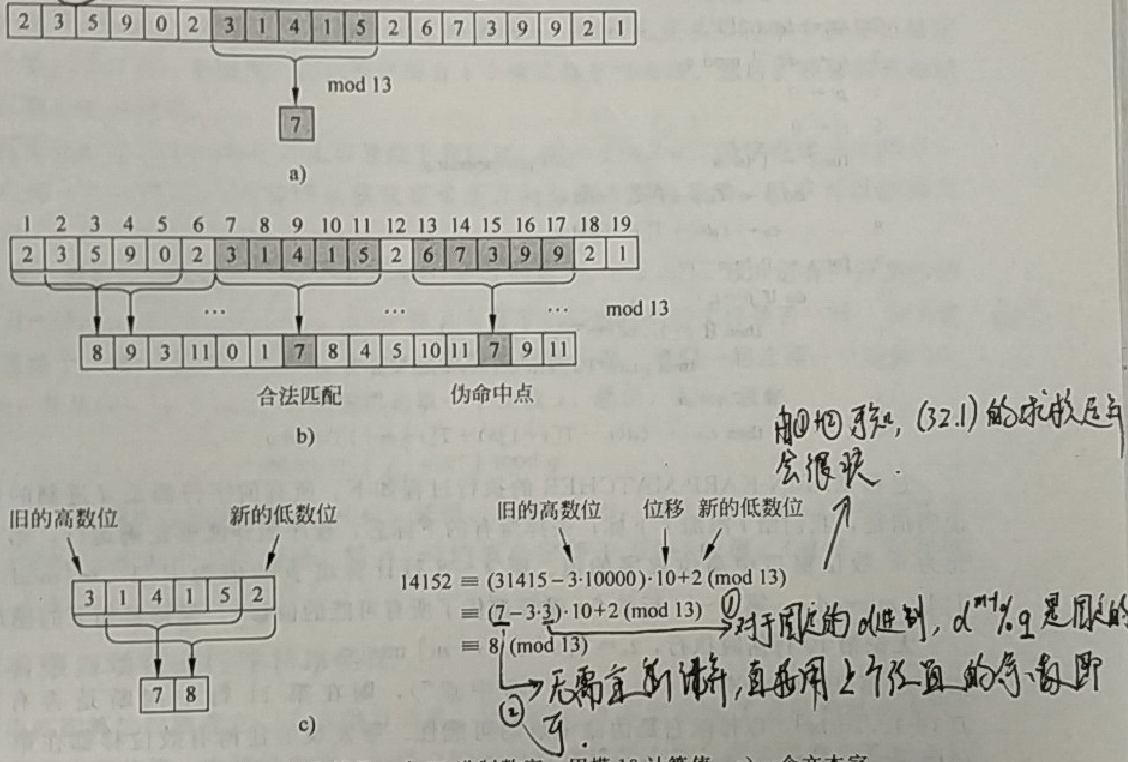
\includegraphics[height=7cm,width=10cm]{notes/algorithm/pic/Rabin-Karp.png}
    \caption{Rabin-Karp示例}
\end{figure}


\section*{有限自动机}
用于字符串匹配的自动机均非常有效: 它对每个文本字符仅检查一次, 并且检查每个文本字符的时间为常数. \\
时间耗费主要在构造自动机上, 为$O(m^3|\sum|)$(优化后可达到$O(m|\sum|)$); 而在检测阶段的时间仅为$\Theta(n)$. 其中$m,n$表示模式$P$,文本$T$的长度,$\sum$为文本域字符集

有限自动机定义: 一个有限自动机$M$是一个5元组$(Q,q_0,A,\sum.\delta)$, 其中:
\begin{itemize}
\item $Q$是状态的有限集合
\item $q_0 \in Q$是初始状态
\item $A \subseteq Q$是一个可接受状态集合
\item $\sum$是有限的输入字符集
\item $\delta: Q×\sum \to Q$的函数, 称为$M$的转移函数
\end{itemize}
在匹配阶段$M$始于状态$q_0$, 每次读入输入字符串$T$的一个字符. 若$M$在状态$q$时读入了输入字符$a$, 则它从状态$q$变为状态$\delta(q,a)$. 每当其当前状态$q$属于$A$时, $M$就接受了迄今为止所读入的字符串, 反之则称为``拒绝的输入"

符号标记:
\begin{itemize}
    \item $\phi: \sum* \to Q$: 终态函数. $\phi(\omega)$表示$M$在扫描字符串$\omega$后终止的状态, 其递归关系式(\ref{eq:zhongtai}) \
    \begin{equation}
        \begin{split}
            \phi(\epsilon) &= q_0, \text{其中}\epsilon\text{表示空字符串} \\
            \phi(\omega a) &= \delta(\phi(\omega), a), \text{其中}\omega \in \sum*, a \in \sum
        \end{split} \label{eq:zhongtai}
    \end{equation}
    \item $\omega \sqsupset x$: 说明字符串$\omega$是$x$的后缀,即$x=y\omega$, 其中$y$为任意字符串
    \item $\omega \sqsubset x$: 说明字符串$\omega$是$x$的前缀
    \item $\sigma: \sum* \to \{0,1,\dots,m\}$, 即 \
        \begin{equation}
            \sigma(x) = \max\{k | P_k \sqsubset \wedge P_k \sqsupset x\}
        \end{equation}
        即$P$的每个前缀$P_k$中可作为$x$后缀的那个所对应的长度$k$即为$\sigma(x)$
\end{itemize}

\section*{KMP}
